\subsection{Stacking}

Trainiert man mehrere Klassifikatoren in einem Ensemble, so müssen in diesem Kontext   Entscheidungen bezüglich der Architektur des Ensembles und der Verwertung der predictions der einzelnen Klassifikatoren getroffen werden.

Eine Möglichkeit, die Ergebnisse mehrerer Klassifikatoren miteinander zu verbinden, besteht in der Stacked Generalization, auch Stacking genannt. Effektiv geht es hier darum, dass die predictions der einzelnen Klassifikatoren, den first-level classifiers, von einem weiteren Klassifikator, dem second-level classifier, zur endgültigen prediction verwertet werden. 

Im Wesentlichen werden dabei in einem ersten Schritt mithilfe des data sets $X = \{x_1, .. ,x_n\}$ mit zugehörigen labels $\{y_1, .. ,y_n\}$ die first-level classifiers $p_1, .. p_K$ trainiert. Deren Ergebnisse $\{(p_1(x_i), .. , p_K(x_i)) \mid x_i \in X\}$ bilden zusammen mit den ursprünglichen labels $\{y_1, .. ,y_n\}$ eine neue Menge, die als das feature set des second-level classifiers verwendet werden kann. [Quelle im Kommentar] %https://books.google.de/books?id=nwQZCwAAQBAJ&lpg=PA500&dq=stacking+classifier+subsets&pg=PA499&redir_esc=y#v=onepage&q&f=false
Der dann resultierende second-level classifier lernt sozusagen, wie die predictions der einzelnen first-level classifier in bestimmten Situationen gewichtet werden sollten, um eine möglichst gute prediction of the whole ensemble zu generieren. Verglichen mit Bagging und Boosting werden hier also nicht die einzelnen Klassifikatoren selbst bezüglich ihrer predictions bewertet und fest von vornherein gewichtet, sondern ihr Einfluss kann je nach Situation variieren. Dieser Vorteil spiegelt sich auch in Klassifikationsergebnissen wider. 


\begin{figure}[H]
	\begin{center}
		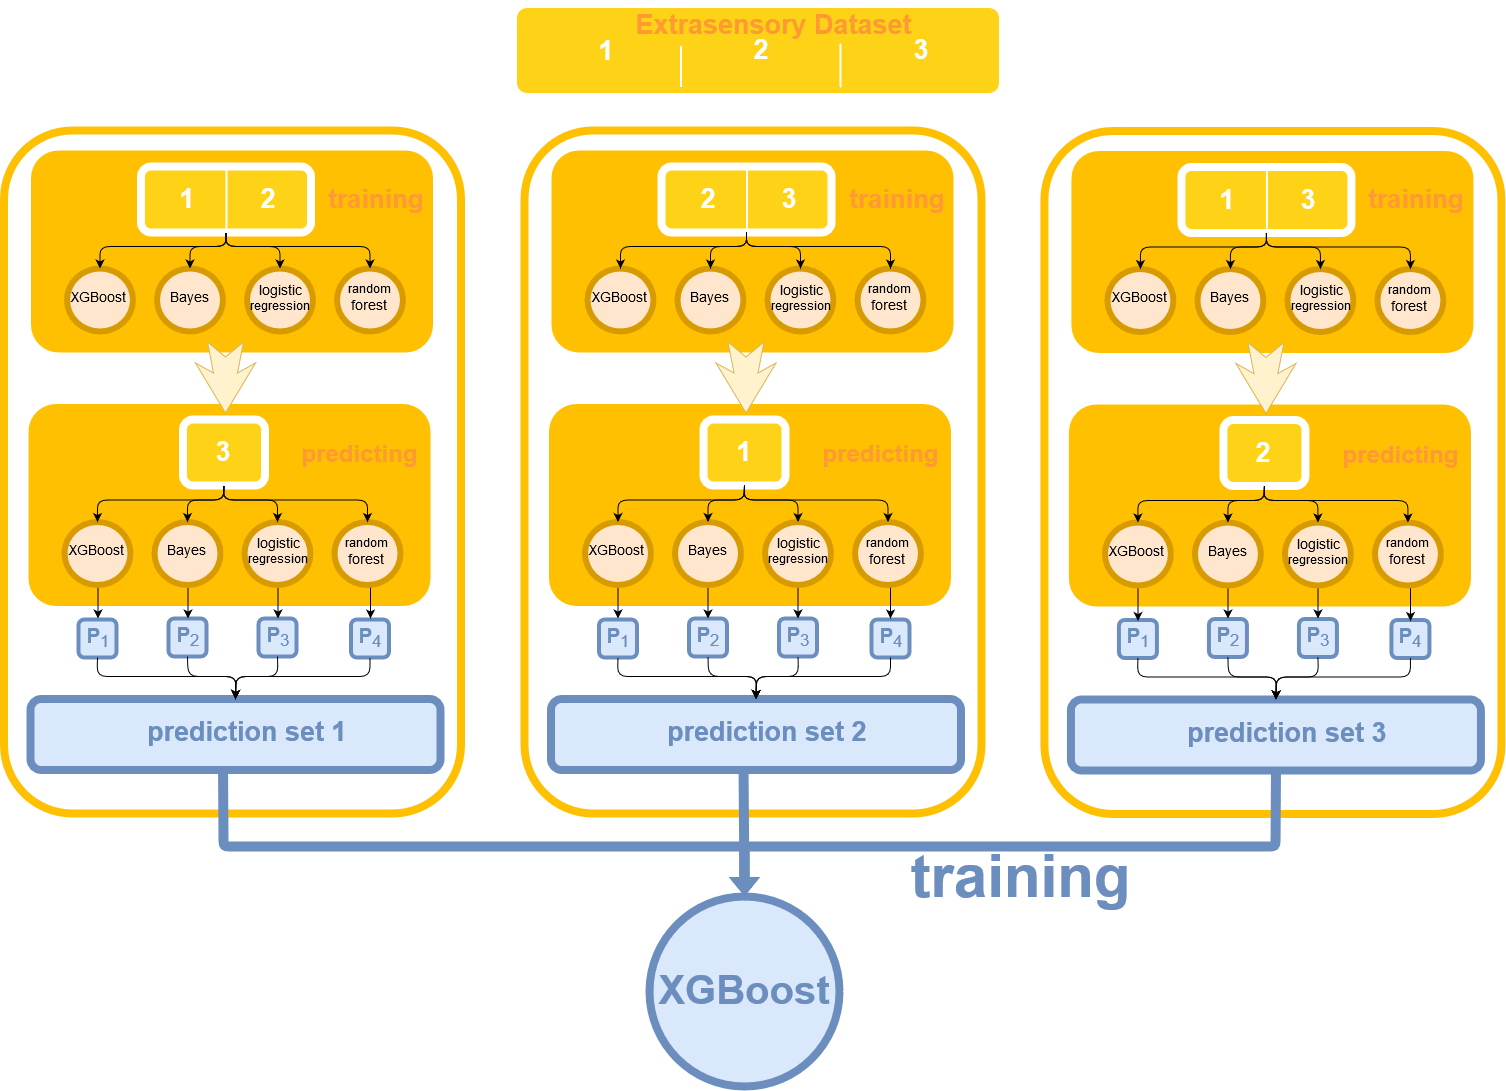
\includegraphics[width=\textwidth]{images/stacking_diagram.png}
		\caption{A Stacking Visualization}
		\label{abb:stacking}
	\end{center}		
\end{figure}	

In unserem konkreten Fall verwendeten wir als first-level Klassifikatoren XGBoost, einen naive bayes Klassifikator, einen random-forest Klassifikator und einen linear regression classificator und als second-level Klassifikator XGBoost. Wie im Schema Fig. \ref{abb:stacking} dargestellt, wurden die first-level Klassifikatoren mit Prinzip der Cross Validation trainiert, dieses Stacking Verfahren wird auch Cross Validation Stacking genannt, indem das data set gedrittelt wurde, was dann wiederum drei prediction sets ergab. Auf diesen prediction sets, ergänzt um die ursprünglichen labels, fand dann das training des second-level Klassifikators statt.

Die Ergänzung des \textcolor{red}{Cross-Validation} Aspekts gegenüber der 